\documentclass[conference]{IEEEtran}
\IEEEoverridecommandlockouts
% The preceding line is only needed to identify funding in the first footnote. If that is unneeded, please comment it out.
\usepackage{cite}
\usepackage{amsmath,amssymb,amsfonts}
\usepackage{algorithmic}
\usepackage{graphicx}
\usepackage{textcomp}
\usepackage{xcolor}
\usepackage{stfloats}
\usepackage[caption=false, font=footnotesize]{subfig}
\def\BibTeX{{\rm B\kern-.05em{\sc i\kern-.025em b}\kern-.08em
    T\kern-.1667em\lower.7ex\hbox{E}\kern-.125emX}}
\begin{document}

\title{Estimating Subgraph Generation Models to Understand Large Network Formation}

\author{\IEEEauthorblockN{1\textsuperscript{st} Laurens Bogaardt}
\IEEEauthorblockA{\textit{Netherlands eScience Center} \\
Amsterdam, the Netherlands \\
l.bogaardt@esciencecenter.nl}
\and
\IEEEauthorblockN{2\textsuperscript{nd} Frank W. Takes}
\IEEEauthorblockA{\textit{University of Amsterdam}\\
Amsterdam, the Netherlands\\
takes@uva.nl}
}

\maketitle

\begin{abstract}
Recently, a new network formation model was proposed. The current research looks into a method to estimate the parameters of this model based on the subgraph census.
\end{abstract}

\begin{IEEEkeywords}
Networks, Graphs, ERGM, SUGM, Subgraphs
\end{IEEEkeywords}

%- given that it is an eScience conference, I think it would be good to balance method and domain a bit better, and add a sentence or 3 about the context of all this:
% - why network science needs these models
% - what social scientists in particular use these models for
% - what researchers in corporate networks use these models for (1 example)
%- make explicit what the main problem is that you are trying to solve, in an eScience context. I think something along the lines of: in computational social science we typically have large network datasets of thousands or millions of nodes; methods to model the formation of these networks only work for small graphs, attempts at scaling these models have been proposed, but are not available as software packages; we develop a methodology for such as package.

Social scientists often aim to understand the incentives and mechanisms which result in large scale structures. Key to this is network formation analysis. However, large datasets are not uncommon, leading to a computational challenge. For example, political scientists interested in global networks of corporate control have to analyse millions of companies.

\begin{table*}[b]
\def\arraystretch{1.5}
\caption{Probabilities in the Subgraph Census}
\begin{center}
\begin{tabular}{|c|c|c|c|c|}
\hline
\textbf{}&\multicolumn{4}{|c|}{\textbf{Subgraphs of the Undirected Triad Census}} \\
\cline{2-5}
\textbf{Model}&\includegraphics[scale=0.8]{Figure03_1.pdf}&\includegraphics[scale=.8]{Figure03_2.pdf}&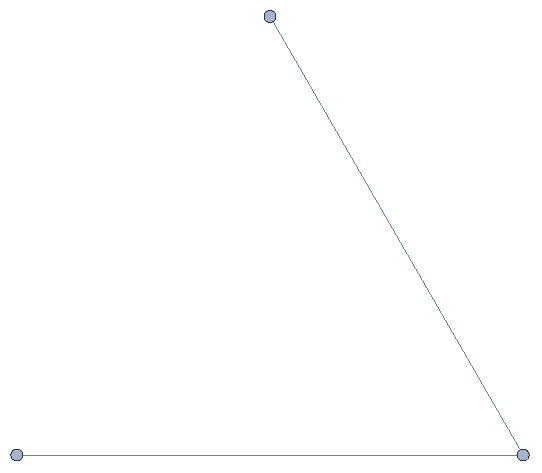
\includegraphics[scale=.8]{Figure03_3.pdf}&\includegraphics[scale=.8]{Figure03_4.pdf}\\
\hline
Links & $p_{L}^{3}$ & $3 \, p_{L}^{2} \, (1-p_{L})$ & $3 \, p_{L} \, (1-p_{L})^{2}$ & $(1-p_{L})^{3}$ \\
\hline
Triangles & $p_{T} \, (p_{T}^{n - 3})^{3}$ & $3 \, p_{T} \, (p_{T}^{n - 3})^{2} \, (1 - p_{T}^{n - 3})$ & $3 \, p_{T} \, (p_{T}^{n - 3}) \, (1-p_{T}^{n - 3})^{2}$ & $(1 - p_{T}) + p_{T} \, (1 - p_{T}^{n - 3})^{3}$ \\
\hline
Links \& Triangles & $p_{T} \, (p_{L} \, p_{T}^{n - 3})^{3}$ & $3 \, p_{T} \, (p_{L} \, p_{T}^{n - 3})^{2} \, (1 - p_{L} \, p_{T}^{n - 3})$ & $3 \, p_{T} \, (p_{L} \, p_{T}^{n - 3}) \, (1 - p_{L} \, p_{T}^{n - 3})^{2}$ & $(1 - p_{T}) + p_{T} \, (1 - p_{L} \, p_{T}^{n - 3})^{3}$ \\
\hline
\end{tabular}
\label{tab:Table1}
\end{center}
\end{table*}

The Exponential Random Graph Model (ERGM) is a frequently used network formation model. However, it suffers from two fundamental flaws. Firstly, its parameter estimates are inconsistent~\cite{Shalizi2013,Chatterjee2013}. Secondly, it does not scale well~\cite{Bhamidi2011}. Recently, an alternative network formation model was suggested: the Subgraph Generation Model (SUGM)~\cite{Chandrasekhar2014,Chandrasekhar2015,Chandrasekhar2016}.

A SUGM is defined by a set of $l$ small subgraphs, such as links, triangles or stars, each with corresponding probabilities. For each subgraph $i$ of $m_{i}$ nodes, the $n$ nodes of the entire network are partitioned into all possible subsets of $m_{i}$ nodes. Then, each of these subsets receives the subgraph $i$ with propability $1-p_{i}$ or remains empty with probability $p_{i}$.

\begin{figure}[htbp]
\begin{center}
\hspace{1mm}
\subfloat{\label{fig:Figure02_1.pdf}\includegraphics[scale=.33]{Figure02_1.pdf}}
\hfill
\subfloat{\label{fig:Figure02_1.pdf}\includegraphics[scale=.33]{Figure02_2.pdf}}
\hspace{1mm}
\caption{The observed network (left) is the union (right) of randomly generated links (red), 2-paths (purple), triangles (green) and 3-stars (yellow).}
\vspace{-5mm}
\label{fig:Figure02}
\end{center}
\end{figure}

The observed network, left in Fig.~\ref{fig:Figure02}, is the union of all these subgraphs, right in Fig.~\ref{fig:Figure02}, where the generated subgraphs may overlap. Multiple neighbouring subgraphs may incidentally form additional structures such as triangles or squares.

The original articles describing SUGM contain two methods to estimate the parameters of the model. The current research suggests a third, more intuitive method based on the subgraph census. In a $k$-subgraph census, a network of $n$ nodes is partitioned into all possible subsets of $k$ nodes, which are then tallied according to their isomorphism class~\cite{Davis1972,Holland1970,Holland1976}.

Table~\ref{tab:Table1} contains the probabilities of observing any of the possible triads for three different generation models. In general, each of the $r$ counts of the census $x_{j}$, together with the probability functions $f_{j}(\hat{p}_{1},\cdots,\hat{p}_{l})$, enter into the multinomial probability mass function of~\eqref{eq:Multinomial} to form the likelihood function. This can be used to estimate the parameters of the model and their confidence intervals.
\begin{equation}
\mathcal{L}(f_{1}, \cdots, f_{r} | x_{1}, \cdots, x_{r}) = \frac{\Gamma(\sum_{j} x_{j}+1)}{\prod_{j} \Gamma(x_{j}+1)} \prod_{j=1}^{r} f_{j}^{x_{j}}
\label{eq:Multinomial}
\end{equation}

Future work should extend the list of possible subgraphs, deal with the correlations within the census, develop an \mbox{\textit{R}-package} and apply the model to real-world data.

\bibliographystyle{IEEEtran}
\bibliography{Bibliography}

\end{document}
